\documentclass[conference]{IEEEtran}

% The preceding line is only needed to identify funding in the first footnote.
% If that is unneeded, please comment it out.
\usepackage{cite}
\usepackage{amsmath,amssymb,amsfonts}
\usepackage{algorithmic}
\usepackage{graphicx}
\usepackage{textcomp}
\usepackage{xcolor}
\usepackage{hyperref}
\usepackage{placeins}
% \usepackage{orcidlink}
% \hypersetup{ colorlinks, linkcolor={red!50!black}, citecolor={blue!50!black},
%     urlcolor={blue!80!black} } \def\BibTeX{{\rm B\kern-.05em{\sc i\kern-.025em
%     b}\kern-.08em T\kern-.1667em\lower.7ex\hbox{E}\kern-.125emX}}
\begin{document}

\title{Reinforcement Learning Agent for Path Planning with Expert Demonstration}

\author{%
    \IEEEauthorblockN{
        Alan Norkham,
        Mikalus Chalupa,
        Noah Gardner,
        Md Abdullah Al Hafiz Khan,
        Xinyue Zhang,
        and Chih-Cheng Hung
        % \orcidlink{0000-0001-5900-9841}
    }

    \IEEEauthorblockA{
        College of Computing and Software Engineering \\
        \textit{Kennesaw State University}\\
        Marietta GA, USA \\
        \{anorkham, mchalupa, ngardn10\}@students.kennesaw.edu, \\
        \{mkhan74, xzhang48, chung1\}@kennesaw.edu
    }
}

\maketitle
\begin{abstract}
    The problem of path planning is a challenging task for mobile robots. A
    practical example can be seen in the robots commonly employed in warehouses:
    they must navigate to pick up goods and move them to certain locations.
    Therefore, the robot needs a method of moving from an initial location in
    the warehouse to a final location repeatedly. In this paper, we propose a
    technique that allows a robot to path plan in generalized environments, from
    different starting and goal locations. The method is based on a graph
    representation of the environment, and is capable of finding the shortest
    path between two points in the environment. In order to generalize
    appropriately, we show that a neural network is able to effectively choose
    the correct actions to take at each time step in the path planning problem.
\end{abstract}

\begin{IEEEkeywords}
    path finding, deep reinforcement learning, expert demonstration, Dijkstra's
    algorithm
\end{IEEEkeywords}

\section{Introduction}
Autonomous vehicles and mobile robots must be able to navigate in environments
that are not completely known in advance, due to the nature of environments to
have unknown obstacles, such as other mobile objects and unknown terrains.
Effective path planning is required in order to make the most of scarce
resources such as time and energy. Additionally, safety should be considered in
environments where the robot works alongside other mobile objects, especially
humans.

Specifically in path finding, many applications include automotive and
autonomous vehicles, robotics, automated warehousing and video games. While
simulations provide a safe environment for testing and evaluation, it removes
the real-world environmental factors. The major concern for path finding
implementation in the market is safety. As the algorithms mature and society
accepts the novelty technology, the speed and accuracy of the system is highly
important in developing the new systems. We consider three criteria for
efficient path planning: the path planning should always be able to find an
optimal path in a static environment, it must be able to generalize to dynamic
environments, and finally, it must minimize complexity, storage, and computation
\cite{janet_essential_1995}.

\section{Background and Related Work}
The need for path planning is derived from the increasing automation of
navigation. The autonomous agent needs to be able to plan a path based on the
limited amount of information given. This problem is explored by Nair et al. who
use an \textit{long short-term memory} (LSTM) to guide an agent through a
simulated environment \cite{nair_robotic_2020}. Yuan et al. also explore the
problem, but with a novel Gated Recurrent Unit-Recurrent Neural Network, and a
more complex simulation \cite{yuan_novel_2019}.

A* algorithm is considered a mature technology for path finding
\cite{hart_formal_1968}. It implements graph traversal, path finding, and
compares the movement cost against the estimated movement cost. Dijkstra's
algorithm is a best first search algorithm and is an extension of A* that also
attempts to find the shortest path between two nodes. With the advancement of
\textit{multi-layered perceptrons} (MLP), methods that are more efficient have
been found. Nair et al. has shown that LSTM is superior to the A* algorithm
\cite{nair_robotic_2020}.

When reviewing previous work, it is proven that MLP performs well over
traditional techniques and to achieve our criteria requirements performance is a
key consideration. Inoue et al. implemented a Rapidly exploring Random Tree and
LSTM and achieved higher learning and generalized abilities
\cite{inoue_robot_2019}. Khan et al. suggested that LSTM models can be used as
an efficient tool for offline path planning applications \cite{khan_using_2017}.
The implementation of LSTM by Guo et al. increases efficiency, achieve shorter
paths, while avoiding obstacles and adapting to general environments
\cite{guo_fusion_2021}. Siddarth et al. propose a deep learning path planning
algorithm trained with generated paths from the A* algorithm using models such
as CNN, LSTM, and a CNN-LSTM hybrid model \cite{siddarth_path_2021}.

There are also some research in dynamic reinforcement learning environments with
continuous action spaces. Li et al. propose a \textit{deep deterministic policy
    gradient} (DDPG) based algorithm for robotic path planning in a dynamic
environment \cite{li_research_2021}. DDPG has some drawbacks such as slow
convergence, so the authors in \cite{li_research_2021} improve the algorithm by
adding a curiosity algorithm which applies attention to improve exploration
\cite{reizinger_attention_2020}.

Another consideration is the novelty of the type of project being worked on. The
surveys reviewed suggest that most works focus on static and real-time
environment where the dynamic environment is the minority. Implementation of
multiagents in real-time and dynamic environments are also limited. Though our
approach implements a single agent, the aspect of obstacle avoidance can be
applied to our project. Through the above works, we have identified
opportunities to provide scientific benefit to path finding in dynamic
environments \cite{abd_algfoor_comprehensive_2015}.

Reinforcement Learning is a promising technique, especially when coupled with
LSTM. Kyaw et al. has shown that \textit{reinforcement learning} (RL) is a
simplistic implementation of the agent maximizing the expected reward objective
and exploring multiple routes \cite{kyaw_coverage_2020}. Not only is LSTM highly
effective with RL, but more recent papers have found that applying RL and Expert
Demonstration with Deep Q-learning, provides decreased training speed and
increased performance in navigating safely and time-efficiently
\cite{liu_improved_2021}. Other studies that have compared the use of
Q-learning and showed that it outperformed other similar algorithms in the
context of games \cite{hester_deep_2017}.

\section{Methodology}

\begin{figure}
    \centering
    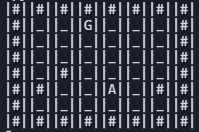
\includegraphics[width=0.3\textwidth]{assets/environment.png}
    \caption{An example state of our environment. $\_$ represents an empty
        space, A represents the agent, G represents the goal, and $\#$
        represents obstacles.}
    \label{fig:path_planning_methodology}
\end{figure}

The environment is an orthogonal grid of cells. A cell can contain either an
agent, an obstacle, the goal, or be empty. The environment size can be varied,
but is fixed to 8x8 grid size for all of our experiments, and the perimeter of
the environment consists of obstacles. The border results in an effective
movement area of 6x6 cells. Initialization of the environment consists of
specifying starting positions of the goal and agent, and any obstacles. Our
experiments focus on three types of starting conditions. The first and simplest
scenario is fixed starting position for both the agent and the goal. The second
scenario keeps the goal fixed, but randomly places the agent. The third, most
complex scenario keeps the goal fixed, places the agent randomly, and adds three
obstacles with random placements. All randomly placed elements are moved to a
random location every training round.

The agent can move in the four orthogonal directions, as long as the space is
empty. If the space the agent is trying to move into is occupied, the agent will
remain at its original position. In the course of a training session, the agent
has 20 steps to make its moves. This number of steps was selected to minimize
the training time spent with the agent attempting to move into a wall or
otherwise not exploring the environment in an attempt to reach the goal.

\begin{figure}
    \centering
    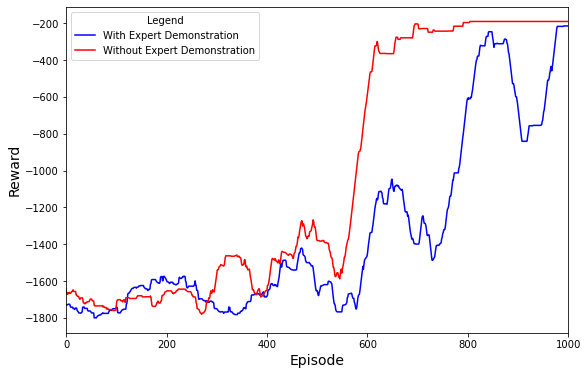
\includegraphics[width=0.5\textwidth]{assets/expertdemonstration.png}
    \caption{Plot for reward recieved by agent after 1000 episodes.
        We show the agent's performance both with and without expert demonstration.
        This experiment is run with fixed-position agent and goal position.}
    \label{fig:expertdemonstration}
\end{figure}

When \textit{deep q-network} (DQN) model is first initialized and training is
started, it will spend large number of rounds exploring the environment with no
concept of the goal. Using expert demonstration, the model can be shown the
desired behavior and receive some pretrained weights this way. For this purpose,
we propose running Dijkstra's pathfinding algorithm before starting a training
session to gather moves and experiences for the model. By running Dijkstra's
algorithm on a generated environment, we can obtain a series of optimal actions
to reach the goal in the shortest number of steps. Then, we can apply these
actions to the environment to receive a set of experiences to demonstrate to the
agent. When expert demonstration was used on the fixed-position agent and goal
scenario, the model was able to converge and achieve optimal path, while the no
expert demonstration experiment did not. Using expert demonstration can
significantly cut down on training time and increasing expert demonstration
rounds will decrease training time accordingly.

Appropriate reward structure is key to a successful reinforcement training
model. Over the course of a training episode, the agent will accumulate rewards
according to the actions it takes. The only positive reward for this scenario is
reaching the goal, which is rewarded by 10 points. Any other move is penalized
by either $-1$ point for moving into free space, or by $-10$ for attempting to
move into an obstacle. The movement penalty is designed to incentivize moving
into the goal tile as soon as possible and the obstacle move penalty attempts to
teach the agent to only move into free tiles. The penalty is further multiplied
by the time-step. This means that the longer the agent takes to find the goal
tile, the more severe the penalty is.

\FloatBarrier
\section{Experimental Results}
Three experiments were run, an environment with fixed-position agent and goal
position, an environment with fixed goal position and random agent position, and
an environment with fixed goal position, random agent position, and three
randomly placed obstacles. Additionally, the environment was limited to an 8x8
grid with a wall of obstacles around the edge of the environment.

The simplest environment with fixed-position agent and goal position was run in
two configurations - with expert demonstration and without expert demonstration.
Including a ten thousand round expert demonstration our Dijkstra's
algorithm-based agent decreased the overall convergence time and allowed the
agent to overcome the local reward maximum of moving back and forth faster. Figure
\ref{fig:expertdemonstration} shows an experiment with and without expert
demonstration. Each line has a moving average window of 70 episodes.

\begin{figure}
    \centering
    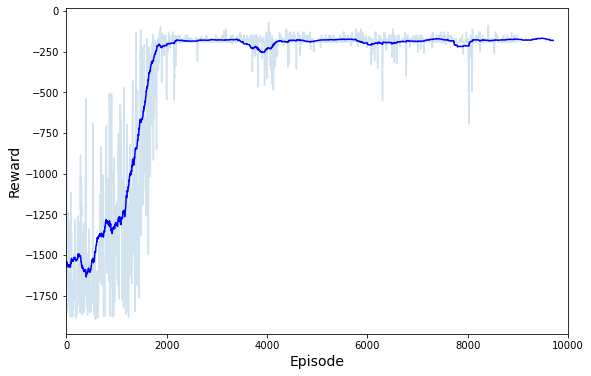
\includegraphics[width=0.5\textwidth]{assets/randomstartnoobs10kep.png}
    \caption{Plot for reward received for 20,000 episodes. This experiment
        included expert demonstration for 10,000 episodes, random agent starting
        location, and no obstacles.}
    \label{fig:randomstartnoobs10kep}
\end{figure}

The second environment is the same as the first experiment, except the agent has
a random starting position. When the environment is generated, the agent is
placed in a random empty position. The goal of this experiment was to increase
the complexity of the environment slightly and evaluate the performance of the
agent.  Figure \ref{fig:randomstartnoobs10kep} shows the results of the second
experiment with expert demonstration. The plot for this experiment contains two
lines, where each line depicts a moving average of the reward recieved. The
faded line has a moving average window of 10 episodes. The solid line has a
moving average window of 300 episodes.

\begin{figure}
    \centering
    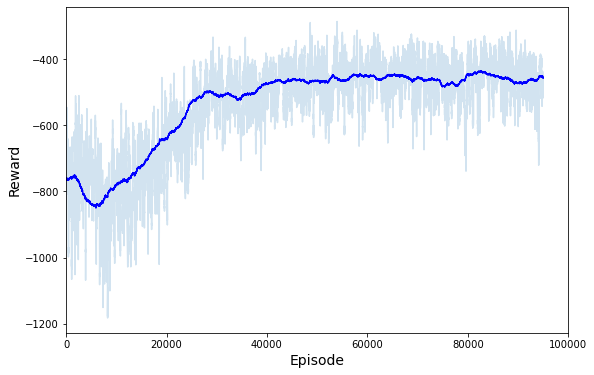
\includegraphics[width=0.5\textwidth]{assets/randomstartrandomobs100kep.png}
    \caption{Plot for reward received for 100,000 episodes. This experiment
        included expert demonstration for 10,000 episodes, random agent starting
        location, and three randomly placed obstacles.}
    \label{fig:randomstartrandomobs100kep}
\end{figure}

The third experiment extends the second experiment by adding three randomly
placed obstacles. The other features of the environment remain the same: the
agent has a random starting position, and the goal position is fixed. Figure
\ref{fig:randomstartrandomobs100kep} shows the results of the third experiment
with expert demonstration. The plot for this experiment also contains two lines.
The faded line has a moving average window of 100 episodes. The solid line has a
moving average window of 5,000 episodes. We also ran this experiment again for
200,000 episodes, shown in Figure \ref{fig:randomstartrandomobs200kep}. When we
ran the training agents for 200,000 episodes, we found that the agent learned a
policy where it recieved a higher average reward. We inspected the 100,000
episode agent's policy and found that the policy it learned tended to move back
and forth. For example, the agent would move \textit{right}, \textit{left},
\textit{right}, and so on for several episodes before moving towards the goal.
We believe by training the model for longer episodes the agent was able to move
past this local minima behavior.

\begin{figure}
    \centering
    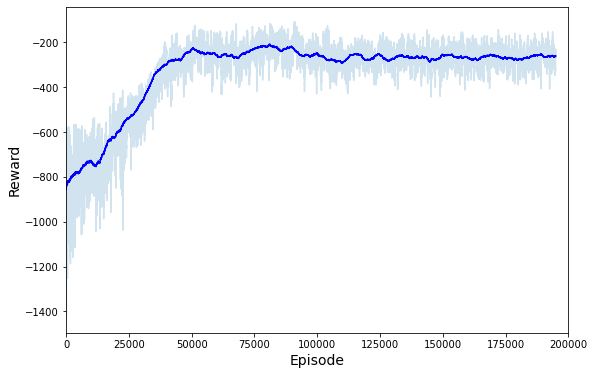
\includegraphics[width=0.5\textwidth]{assets/randomstartrandomobs200kep.png}
    \caption{Plot for reward received for 200,000 episodes. This experiment
        included expert demonstration for 10,000 episodes, random agent starting
        location, and three randomly placed obstacles.}
    \label{fig:randomstartrandomobs200kep}
\end{figure}

There are some drawbacks to our approach. The first drawback is that the
randomly initialized environment is complex but has a small state space.
Additionally, we use float representation of the different objects in the
environment which has a smaller observation dimensionality than standard color
representation for 2-d reinforcement learning environments. A higher dimensional
state space may be desirable for an agent to learn to navigate the environment.
The second drawback is that the action space is discrete and limited to four
actions. A robot with a continuous action space would be a more appropriate
model in a live environment. The third drawback is that the expert demonstration
with Dijkstra's algorithm always takes the correct action. Therefore, the agent
may have trouble learning the incorrect actions, which are just as important for
the agent to judge the value of each action. Additionally, Dijkstra's algorithm
is computationally expensive in larger environments.



\FloatBarrier
\section{Conclusion}
In conclusion, we presented a custom environment and applied a DQN agent to
learn a policy to complete the task. We used expert demonstration with
Dijkstra's algorithm to generate a set of optimal actions to reach the goal in
the shortest number of steps. Due to the flexibility of our custom environment,
we analyzed the performance of the agent with a variety of different starting
positions and obstacles. We found that our environment is somewhat complex when
random positions for the agent and obstacles are used. In future work, we would
like to experiment with different parameters for our expert demonstration. Since
the expert always takes the correct action, the agent might not learn why the
incorrect actions are not taken and therefore have a limited decision making
ability. This might explain why in our first experiment the agent without expert
demonstration settled into a local optimal policy while the agent with expert
demonstration did not.

\bibliographystyle{IEEEtran}
\bibliography{main}
\end{document}